\documentclass[11pt]{article}

\usepackage{geometry}
\geometry{hmargin=2.5cm,vmargin=1cm}

%% Load packages %%
%\usepackage[applemac]{inputenY}
\usepackage[english]{babel}
\usepackage[utf8]{inputenc}
\usepackage{graphicx}
\usepackage{float}
\usepackage{amsmath}     % Mathematical writing
\usepackage{amssymb}
\setlength{\parindent}{0pt}

\usepackage{subfig}

\usepackage{listings}

\usepackage{amsmath}
\DeclareMathOperator*{\argmax}{argmax} % thin space, limits underneath in displays


\title{Practical 1 - Speech commands}
\author{Yonatan DELORO}

\begin{document}

\maketitle

\section{MY QUESTIONS FOR THIS TP}

0. WRITE AS A RESEARCH REPORT ??

1. Improve parameters of Melfilters/MFCC

4. Trigram. Complexify Viterbi much. Is is it penalized if not ?

2. Melfiter better for CNN ? (MFCC suggested for part II)

3. Bigram. We modify if 0 of (i,j) but if low should we modify too ?

5. Confirm what is beam search.

6. Normalize across time ??

\section{I. Classification of single voice commands}

No question. CF. code

\paragraph{Speech features}

First of all, as we aim at classifying single English words, we are not interested in features caraterizing the pitch but only in the features defining the vocal tract (and not the glottal source). Hence the MFCC features can appear a priori as a better option than the Mel-filterbanks. However, we will see that our experiments will not end up with such a conclusion for each discrimative model assessed.

Secondly, the speech features in the 2d- time/frequency domain (with mel-filterbanks or MFCC coefficients on the the frequency axis) were flattened into a 1d-vector in the initial code. I chose to keep these features as a 2d array, and to flatten these only if the discriminative model used for classification could not handle 2d-inputs. Indeed, we will for instance CNN as a classification model, which seem well-suited for multi-dimensional arrays. I modified the padding functions adequately, choosing 101 as for min-len parameter (minimal length of the recordining).

%https://www.researchgate.net/post/How_can_I_give_speech_data_as_input_to_a_convolutional_neural_network

\textit{The parameters of the speech features such as the min/max frequency or window size are poorly chosen, look inside the resources mentioned in the class to find the best parameters for mel-filterbanks and MFCC.}

\begin{figure}[h!]
\begin{center}
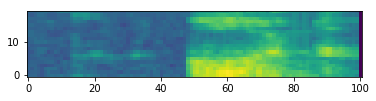
\includegraphics[scale=0.5]{i.png}
\caption{Mel-filterbank features for a sample of word " ".}
\end{center}
\end{figure}

\begin{figure}[h!]
\begin{center}
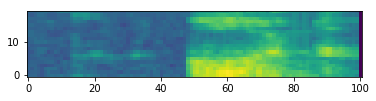
\includegraphics[scale=0.5]{i.png}
\caption{MFCC features for a sample of word " ".}
\end{center}
\end{figure}


\paragraph{Classification models} Three type of models were tried : 

\textbf{(i) Logistic Regression (LR)} A first proposal for this multi-label classification problem is to perform a logistic regression on the flattened speech features for each word class against all others. Each data is then labelled with the class obtaining the largest probability. I added a l2 regularization term to the cross-entropy loss of the LRs to allow for better generalization. In other words, the loss to be optimized for each of the $30$ LR is : $\mathcal{L}(x_i,y_i) = - \sum_{i=1}^N y_i \log \sigma(w x_i) + (1-y_i) \log (1-\sigma(w x_i)) + \alpha ||w||^2$, and I used SGD to do so for scaling purposes. I chose the $\alpha$ parameter maximizing the accuracy score obtained on the validation set.

\textbf{(ii) Neural network} Two types of neural networks were investigated : 

\begin{itemize}
\item First, I tried a neural network with fully connected layers, taking as input the 1d-flattened speech features. The best I could get is composed of 2 hidden layers (with 128 and 64 hidden neurons respectively). 
\item Then, I moved to a convolutional neural network taking as input the 2d-flattened speech features treated as images of depth 1. The architecture of the features extractor I ended with is composed of 3 convolutional layers (with increasing number of filters -8,16 and 32- and decreasing size of filters -(11, 5), (7,3) and (3,1)) each conv layer followed by (2,2) maxpooling. Then a bottleneck with one hidden layer (64 neurons) enables to discriminate between the 30 classes.
\end{itemize}
For each layer (dense or convolutional) of both networks, "relu" was choosen as the activation function, except for the last layer to which we applied the "softmax" function, relevant for classification. Categorical cross-entropy loss was optimized with Adam (initial learning rate of 0.001), stopping whenever the validation loss did not decrease for three iterations. I also used dropout (probability of 0.3) after/for hidden dense layers to struggle against overfitting.
\textit{The neural net proposed is a shallow neural net, far from the best you can train. You should try bigger, deeper architectures, different types of regularization, activation functions, learning rate and so on. You can change the** Runtime of your colab instance and use a GPU**.}

To investigate maybe ? RCNN

\begin{figure}[h!]
\begin{center}
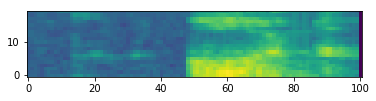
\includegraphics[scale=0.5]{i.png}
\caption{Choice of the regularization weight in the Logistic Regression.}
\end{center}
\end{figure}

\begin{figure}[h!]
\begin{center}
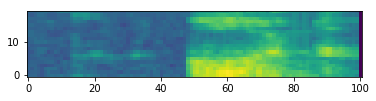
\includegraphics[scale=0.5]{i.png}
\caption{Train and Validation loss throughout the CNN training with and without dropout.}
\end{center}
\end{figure}

\paragraph{Normalization and augmentation}

For better generalization, I also observed the impact of :
\begin{itemize}
\item normalizing the speech features. I notably compared two types of normalization : the standard one, where we center and scale each feature dimension computing mean and variance across the dataset for each timestep ; and the Cepstral Mean Normalization, which consists in centering and scaling each speech feature dimension (on the frequency axis) computing mean and variance over each sample across time.  The theoretical advantage of this second normalization is that we do not assume constant channel conditions among the recordings. However, we will see that in practice the first one will work better given the short size of the recordings (computing mean and variance over the entire dataset gives more accurate estimates).
%Should we prefer the BATCH NORMALIZATION
\item augmenting the original train dataset of 300 instances per class with noisy instances. More precisely, the process of augmentation is the following : I selected a random subset of the $300*30$ waveforms of the train dataset of a given size, and to each of these I added a random sequence extracted from the waveform of one of the $6$ proposed background noises (artificial or real) lasting the same amount of time as the original sample waveform.
\end{itemize}

\textit{A standard way of improving generalization is to do mean-variance normalization on your data set. This is done by computing the mean and variance of each feature dimension on the entire training set, and then use it to normalize train, valid and test set. The dataset provides noises samples, either artificial (pink, white noise) or real (dishes, bike) in the folder backgroundnoise. You can try augmenting your dataset by adding noise to the waveforms before computing the features. The model is only trained on 300 examples per class, if your hardware allows it, try training on more examples}

\subsection{Results}


\begin{table}[h!]
\centering
  \begin{tabular}{|l|l|l|l|l|l|l|}  \hline
    Features  & Discriminative & Features  & Data &  Train  & Validation & Test \\     
   Extraction & Model & Normalization & Augmentation  &  Score & Score & Score \\  \hline    
    Mel-filterbanks & LR & - & - & & &  \\ \hline
    MFCC & LR & - & - & & &\\ \hline
    Mel-filterbanks & MDP & - & - & & & \\ \hline
    MFCC & MDP & - & - & & &\\ \hline
    Mel-filterbanks & CNN & - & - & & &\\ \hline
    MFCC & CNN & - & - & & &\\ \hline
    Mel-filterbanks & CNN & Standard & - & & &\\ \hline
    Mel-filterbanks & CNN & Sample-specific & - & & & \\ \hline
    Mel-filterbanks & CNN & Standard & +100\% (same  & & & \\ 
     &  & & samples with noise) & & & \\ \hline
  \end{tabular}
  \caption{Accuracy score on the train, validation and test set for each pipeline.}
\end{table}

Add time considerations


\textit{You should find the best model by comparing validation accuracies. After you find your best model, finally test it on the test set and print the result. Comment on the results (best model, best features, classes that are the most difficult to recognize).
}
\section{II. Classification of segmented voice commands}

\subsection*{q1.}
$S+D+I$ is positive by definition, and zero when the sequences are perfectly aligned. Therefore, we cannot have WER<0.

However $S+D+I$ can be larger than $N$. For instance the hypothesis sequence can be of length $2N$ and contain no word of the reference sequences, in which case $S+D+I=2N$ (shortest path to align the two sequences is composed of $N$ substitutions and $N$ insertions).
Therefore, we can have WER>100.

\subsection*{q2.}

With such line 

\begin{lstlisting}
elif train_labels.count(label) < nb_ex_per_class:
            fs, waveform = wav.read(full_name)
            train_wavs.append(waveform)
            train_labels.append(label)
\end{lstlisting}            

we ensured that the discriminator of speech commands has been trained with balanced dataset $P(W_i) = constant$.

Therefore, we can rewrite the acoustic model using Bayes rule as :
 \begin{align*}
 P(X_i|W_i) &= \frac{P(W_i|X_i)P(X_i)}{P(W_i)} \\
 & =  \frac{1}{|W|} P(W_i|X_i)P(X_i) \\
 &  \propto P(W_i|X_i)P(X_i) \\
 & \propto P_{\text{discriminator single word}}(W_i|X_i) 
 \end{align*} 
 
 \subsection*{q3.}
 
The greedy decoder assumes full independence between consecutive spoken words : we label each waveform of the sentence with the word label of highest probability for the chosen discriminator model, ie. the convolutional neural network of part I.

Word error rate between "go marvin one right stop" and " go marvin one left stop" is 0.2 as the shortest path to go from one sentence to the other using the three operations(insertions, substitutions, deletions) is 1 : we substitute "right" by "left". Hence WER = 1/5 = 0.2 = 20%.

 
  \subsection*{q4.}
  
  The Bigram appproximation formula of the language model I used is the following :
  
  \begin{align} p(w_2|w_1) &= \frac{C(w_1w_2)}{C(w1)} & if ~ C(w_1)>0 \\
  &= \frac{C(w_2)}{V}  & otherwise
  \end{align}
  
  where $C(s)$ denotes the count number of the string $s$ in the corpus and $V$ the size of the corpus ($V = \sum_{w \in W} C(w)$, where $V$ is the set of speech commands, as the corpus do not contain any other command).
  
  In other words, whenever there is no count of word $w1$, we assume that any speech command $w_2$ has equal chance to appear after it.
  This approximation formula, which corresponds to the maximum likelihood, is not too wrong here as there are only $30^2=900$ bigrams combinations while the training corpus is composed of $ $ (sparsity is not a hard issue there).
  
  \subsection*{q5.}
  
  To build this language model, I computed the number of each unigram, and of each bigram (stored in a vector and in a matrix) reading the texts of the training corpus, which allowed to compute as a second step the probability of each word conditionnally to the previous one thanks to the approximation formula above. We will call this array the transition matrix.
  
  \subsection*{q6.}
  
  If we want to model $P(w_N|w_{N-1},...,w_1)$ with larger $N$, we may end with a model capturing longer-time dependencies between words in a sentence, but we need to face the sparsity problem arising: if the corpus is not large enough, there might be very few counts of $N-$ grams so that the maximum-likelihood estimate :
  
    \begin{align} p(w_N|w_{N-1},...,w_1) &= \frac{C(w_1...w_{N})}{C(w_1...w_{N-1})} & if ~ C(w_1...w_{N-1})>0 \\
  &= p(w_N|w_{N-1},...,w_1)  & otherwise
  \end{align}
  
might become too approximate. A solution proposed in $https://mi.eng.cam.ac.uk/~mjfg/mjfg_NOW.pdf$ is the Katz smoothing which consists in decreasing (with a multiplicative factor less than 1) the ratio $\frac{C(w_1...w_{N})}{C(w_1...w_{N-1})}$ if $C(w_1...w_{N})$ is below a certain amount, and using $ p(w_N|w_{N-1},...,w_2)$ as the estimate whenever $C(w_1...w_{N})$ (not $C(w_1...w_{N-1})$) is 0.
  
  
  \subsection*{q7.}
  
  In beam search algorithm, we are keeping in memory, at each timestep $t$ of the sequence, the $K$ (beam-size parameter) most likely sequences. To do so, we can at each time step $t+1$ : (i) select the $K$ most probable words at timestep $t+1$ given by our discriminative model (the other are suboptimal); (ii) compute the probability of each of the $K$ stored sequences from time $0$ to time $t-1$, followed by each of the $K$ new most probable words; (iii) keep in memory the $K$ sequences from $0$ to $t$ with highest probabilities. As the complexity to select the top $K$ elements in a list of length $N$ is $O(Nl \log(K))$, yhe complexity of the beam search algorithm is therefore : $O(T (N \log K + K^2 + K^2 \log(K))) = \mathbf{O(T \max(N, K^2) \log K))}$ where $T$ is the length of the sequence, $N$ is the number of possible speech commands and $K$ is the beam-size parameter.
  
  \subsection*{q8.}
  
  Let us denote $\phi^t_j$ the probability to be in state $j$  at step $k$, or to be more precise, the probability of the most likely sequence ending with word $j$ at step $k$. Then we have the relationship :
  
  $$\phi^t_j = \max_{j'} \{ \phi^t_{j'} \times p_L(j|j') \} \times p_D(j|s^t) $$
   
   where $p_L$ denotes the bigram language model (probability of the next word given the previous one), $p_D$ the discriminative model (probability of a word given the signal, $s^t$ denotes the waveform at "sentence time" $t$).
   
   The Viterbi algorithm can be implemented by : (i) iterating forward in time to compute $\phi^t_j$ for each possible word $j$ for each $t \in [1,T]$ with $T$ the length of the sentence ("forward pass"), hence we can access to the probability of the most likely sequence $\max_j \phi^T_j$ , (ii) iterating backward in time to access to the words enabling to reach this maximum probability, ie $j_T^*=\argmax_j \phi^T_j$ and $j_t^* = \argmax_{j'} \{ \phi^t_{j'} \times p_L(j_{t+1}^*|j') \}$ for $t \in [1,T-1]$. To do so more efficiently, I also stored during the forward pass $w^t_j = \argmax_{j'} \{ \phi^t_{j'} \times p_L(j|j') \}$ for each $j$.
   
   The complexity of the Viterbi algorithm is therefore $O(T (N^2 + N \log N)) =   \mathbf{O(T N^2)}$ where $T$ is the length of the sequence and $N$ is the number of possible speech commands.
   
   \begin{table}[h!]
\centering
  \begin{tabular}{|l|l|l|l|l|l|l|}  \hline     
   Decoder & Train WER & Test WER & Evaluation time \\  \hline    
   Greedy (no language model) &  &  &  \\ \hline
    Beam search (K=5)  & & & \\ \hline
    Viterbi  & & & \\ \hline
  \end{tabular}
  \caption{Word error rates and computation times for the three decoders, using a subset of the training set, the bigram language model and the CNN discriminative model (with Mel-filterbanks features normalized, and without data augmentation.)}
\end{table}

  \subsection*{q9.}
  
  \begin{figure}[h!]
\begin{center}
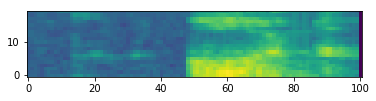
\includegraphics[scale=0.5]{i.png}
\caption{Sentences leading to a higher WER.}
\end{center}
\end{figure}

  \subsection*{q10.}
  
  \subsection*{q11.}
  
\end{document}
